% Standalone research manuscript. Compile twice with xelatex -no-shell-escape.
% All diagrams and bibliography are embedded. No font files are distributed.
\documentclass[11pt,letterpaper]{article}
\usepackage{fontspec}
\setmainfont{Noto Serif}
\setsansfont{Noto Sans}
\setmonofont[Scale=.83]{DejaVu Sans Mono}
\usepackage[margin=.94in,headheight=15pt]{geometry}
\usepackage{amsmath,amssymb,amsthm,mathtools}
\usepackage{microtype,booktabs,tabularx,longtable,array}
\usepackage{enumitem,algorithm,algpseudocode,placeins}
\algrenewcommand\textproc{\textsf}
\usepackage{tikz,xcolor,fancyhdr,titlesec,needspace,listings,etoolbox}
\usetikzlibrary{arrows.meta,positioning,calc,fit}
\usepackage[round,authoryear]{natbib}
\usepackage{xurl,hyperref}
\definecolor{ink}{HTML}{302047}
\definecolor{accent}{HTML}{6743A5}
\definecolor{teal}{HTML}{176E7A}
\definecolor{muted}{HTML}{655E70}
\definecolor{wash}{HTML}{F5F2FA}
\hypersetup{colorlinks=true,linkcolor=ink,citecolor=ink,urlcolor=teal,
 pdftitle={Out-Reflect: Transformational Intelligence for Constructing Self-Correcting Evidence},
 pdfauthor={Vincent Boucher},
 pdfsubject={Moment-shaped audit synthesis; fallible references; error correction; nonlinear scope; SUCCESSOR Omega},
 pdfkeywords={transformational intelligence, self-correcting evidence, polynomial audit, coded experiments, reference corruption, SUCCESSOR Omega}}
\urlstyle{same}
\pagestyle{fancy}\fancyhf{}
\fancyhead[L]{\small\sffamily OUT-REFLECT}\fancyhead[R]{\small Boucher}
\fancyfoot[C]{\small\thepage}\renewcommand{\headrulewidth}{.35pt}
\setlength{\parindent}{1.1em}\setlength{\parskip}{.14em}
\setlength{\emergencystretch}{2em}\setlength{\tabcolsep}{5pt}
\renewcommand{\arraystretch}{1.12}
\titleformat{\section}{\large\bfseries\color{ink}}{\thesection}{.65em}{}
\titleformat{\subsection}{\normalsize\bfseries}{\thesubsection}{.65em}{}
\titlespacing*{\section}{0pt}{1.1em}{.45em}
\titlespacing*{\subsection}{0pt}{.75em}{.25em}
\setlist{nosep,leftmargin=1.5em,topsep=.25em}
\newcolumntype{Y}{>{\raggedright\arraybackslash}X}
\newcolumntype{P}[1]{>{\raggedright\arraybackslash}p{#1}}
\renewcommand{\topfraction}{.95}\renewcommand{\bottomfraction}{.85}
\renewcommand{\textfraction}{.06}\renewcommand{\floatpagefraction}{.85}
\newcommand{\R}{\mathbb R}\newcommand{\V}{\mathcal V}\newcommand{\N}{\mathcal N}
\newcommand{\Om}{SUCCESSOR~$\Omega$}
\newcommand{\rank}{\operatorname{rank}}\newcommand{\supp}{\operatorname{supp}}\newcommand{\vecop}{\operatorname{vec}}
\newcommand{\insight}[1]{\begin{center}\setlength{\fboxsep}{9pt}\fcolorbox{ink}{wash}{\begin{minipage}{.92\linewidth}#1\end{minipage}}\end{center}}
\newcommand{\mirror}{
\begin{tikzpicture}[x=.32cm,y=.32cm,baseline=-.06cm,line width=.85pt,draw=accent]
\draw[fill=wash] (0,1.6) ellipse (.85 and 1.3);
\draw (0,.3)--(0,-.5);\draw (-.6,-.5)--(.6,-.5);
\draw[draw=teal] (-.42,1.25)--(.28,2.18);\draw[draw=teal] (-.13,.98)--(.45,1.75);
\end{tikzpicture}}
\newtheorem{definition}{Definition}[section]
\newtheorem{proposition}{Proposition}[section]
\newtheorem{theorem}{Theorem}[section]
\newtheorem{corollary}{Corollary}[section]
\theoremstyle{remark}\newtheorem{remark}{Remark}[section]
\BeforeBeginEnvironment{theorem}{\Needspace{9\baselineskip}}
\BeforeBeginEnvironment{proposition}{\Needspace{8\baselineskip}}
\lstset{basicstyle=\small\ttfamily,breaklines=true,columns=fullflexible,keepspaces=true,
 showstringspaces=false,frame=single,rulecolor=\color{muted},aboveskip=.6em,belowskip=.6em}
\newcommand{\Pset}{\mathcal P}\newcommand{\Fset}{\mathcal F}\newcommand{\Qop}{\mathcal Q}
\newtheorem{lemma}{Lemma}[section]
\begin{document}
\thispagestyle{plain}
\begin{center}
{\small\sffamily\color{accent} MONTREAL.AI\quad /\quad TRANSFORMATIONAL INTELLIGENCE $\infty$\par}
\vspace{.75em}
{\fontsize{40}{44}\selectfont\bfseries\color{ink} Out-Reflect\hspace{.3em}\mirror\par}
\vspace{.65em}
{\Large\bfseries Transformational Intelligence for\par}
\vspace{.15em}
{\Large\bfseries Constructing Self-Correcting Evidence\par}
\vspace{.9em}
{\large Vincent Boucher\par}
{MONTREAL.AI\par}
{Montréal, Québec, Canada\par}
\vspace{.45em}
{21 October 2026\quad$\cdot$\quad Substantively revised research edition\par}
\end{center}
\begin{abstract}
An evaluator can be complete inside the wrong program class, and a reference answer can be the error it should expose. We make both limitations constructive. Instead of requiring every individual verdict to be trustworthy, we design experiments whose joint structure identifies a supported transformation despite bounded corruption of their results. The new technical object is a moment-shaped audit code. For $n\ge4$ observations, $m=k(n-1)$ channels, centered input $C$, and cubic invariant $s(C)=\sum C_{ij}^{3}$, consider the nonlinear family $F(C)=\sum_{\ell=0}^{L}s(C)^\ell C B_\ell$. We construct rational inputs that make $s(C)$ follow a prescribed power while preserving a full-rank contrast frame. Their normalized outputs become polynomial evaluations of the unknown coefficient blocks. Together with inherited balanced probes, they form a nested, distance-certified audit. Exactly $k(L+1)+2t$ fixed full-output reference calls are necessary and sufficient to recover every member of this class when at most $t$ entire records are arbitrarily wrong. The result is a class-specific synthesis theorem built on established error correction, not a new coding principle. In the executed eight-row, twenty-one-channel case, the original three probes cannot expose a quartic impostor. Five constructed additions both reveal it and recover all 882 coefficients while locating one corrupted reference response. Every possible single-record position is exercised with four error forms. A three-generation sequence enlarges supported polynomial degree from one to four to seven using five, eight, and eleven cumulative calls; a genuine target change instead invalidates two old expected outputs. Source-group and beyond-budget counterexamples prevent record redundancy from being mistaken for independent truth. The advance is from checking within a supplied reliable mirror to constructing a bounded evidence system that can repair the mirror's scope and one of its observations. No universal self-certification, neural improvement, or operational deployment is established.
\end{abstract}
\noindent\textbf{Keywords:} transformational intelligence; reflective verification; coded experiments; nonlinear identification; fallible references; evidence inheritance; SUCCESSOR $\Omega$.
\begin{center}\small
\textbf{Find your Alpha. Build your SUCCESSOR $\Omega$.}\par
\href{https://github.com/MontrealAI/AGI-Alpha-Agent-v0}{github.com/MontrealAI/AGI-Alpha-Agent-v0}
\end{center}
\clearpage

\section{The next mistake may be in the evidence}
An AI proposes a scientific data transformation. Its outputs have the right means. Reordering observations reorders the result correctly. Every retained reference example passes. The judge reports success.

There are at least two different ways this apparent success can be false. The candidate may exploit a behavior the examples never excite. Or a reference result used to judge the candidate may itself be wrong. Asking a second model to agree with the first does not necessarily distinguish either failure. Repeating one reference service does not make its systematic error independent.

The first edition of \emph{Out-Reflect} constructed missing tests within a declared linear class. Its two most consequential counterexamples remained outside its positive guarantee: a nonlinear impostor passed the finite fixtures, and a corrupt reference could define a coherent but wrong target \citep{reflect1}. Those were not minor caveats. They identify the next object to invent.

\insight{\textbf{Do not require every reflection to be right. Construct evidence in which a bounded wrong reflection can be located and corrected.}\par\smallskip The purpose remains fixed. The evaluator's scope and its dependence on individual reference answers become editable.}

The foundational distinction between purpose and inherited means remains binding \citep{transform}. This revision constructs that object for an explicit nonlinear program family. The experiments are not interchangeable votes. Each poses a different algebraically related question. Their answers form a codeword: a collection with enough enforced relationships that an erroneous answer cannot generally imitate a different valid transformation without contradicting too many other records. The reflection system recovers a supported target, identifies inconsistent records, and produces a concrete counterexample to a bad candidate.

The essential new construction is not simply to attach Reed--Solomon terminology to a test suite. It is to design actual admissible inputs whose nonlinear responses have the coding structure required for recovery. We shape a third moment while preserving a full-rank observation frame. This converts a particular nonlinear verification problem into an exact coefficient-recovery problem, preserves the predecessor's real probe inputs, and supports deliberate enlargement of the candidate language.

\subsection{What changes, immediately}
In the anchor, a candidate adds a cubic-moment-dependent channel transformation to the intended linear calibration. It still passes all three old numerical fixtures because their cubic moments are zero. The earlier exact linear-class checker would correctly refuse this candidate as unsupported; the new paper does \emph{not} pretend that the earlier conditional theorem approved nonlinear code.

The stronger response is neither to waive the class restriction nor to stop permanently at that refusal. A bounded program normalizer identifies the extra polynomial term. The constructor enlarges the supported audit, reuses the three original input--output records, and generates five additional inputs. One of the five new reference answers is deliberately replaced by the impostor's own answer. All eight are then supplied, without the corrupted location, to the recovery procedure.

It recovers the intended transformation exactly and identifies the inconsistent record. The reference corruption is not an easy nonzero-mean anomaly: the substituted answer is itself a zero-mean output of another admissible nonlinear program.

\begin{table}[htbp]\centering\small
\caption{The stronger task and its executed resolution. ``Record'' means one complete $8\times21$ response, not a scalar measurement.}\label{tab:opening}
\begin{tabularx}{\linewidth}{@{}YP{.40\linewidth}@{}}\toprule
Question & Result in the revised construction\\\midrule
Can the nonlinear impostor pass the original three numerical probes? & Yes; all their cubic moments vanish.\\
Does the original linear certificate apply to that impostor? & No; its class gate must refuse it.\\
What new evidence is constructed? & Five additional moment-shaped inputs; eight total records.\\
What is allowed to be wrong? & Any one complete reference-response record.\\
What is recovered? & Both $21\times21$ coefficient matrices: 882 coefficients.\\
What happens to the wrong reference? & Its record is located; the supported target is recovered.\\\bottomrule
\end{tabularx}
\end{table}

The result does not authenticate an unlimited number of mutually consistent false references. It replaces a stronger assumption---every supplied reference value is right---with a different, explicit assumption: the true target is in the admitted family and at most one record is corrupted. That assumption must itself be justified by a real deployment. The construction makes its consequences and failure boundary checkable.

\subsection{A substantive revision, not a more emphatic introduction}
Three changes carry the paper. First, the nonlinear failure from the earlier edition becomes part of a positively supported program family. Second, the reference transcript can contain bounded adversarial errors rather than being uniformly trusted. Third, the audit can grow without re-acquiring unchanged observations, while separately detecting when a changed target makes old expected outputs obsolete.

The broader research sequence provides the purpose discipline. \emph{Out-Think} makes an internal representation replaceable; \emph{Out-Strategise} changes what success requires the system to know; \emph{Out-Execute} separates retained work from a new commitment \citep{think,strategy,execute}. Here reflection changes the organization of evidence itself. It inherits verified records without inheriting an unconditional right to believe them in every new scope.

\section{A verdict is not the same object as evidence}
\label{sec:distance}
Let $\Fset$ be a declared set of target programs. A fixed audit chooses probes $X_1,\ldots,X_q$ before receiving their results. Its clean transcript is
\begin{equation}
 \mathcal A(F)=\bigl(F(X_1),\ldots,F(X_q)\bigr).
\end{equation}
Each entry may be a vector or matrix. A bad record can replace the entire entry by arbitrary data of the expected shape. Errors need not be independent or random. At most $t$ records are bad; all other records equal the same fixed target's exact response. A missing or explicitly untrusted record can instead be treated as an erasure under a separately specified budget.

The purpose need not require identifying the whole target. Let $\Qop(F)$ be the output or property that actually matters. Define its audit distance by
\begin{equation}
 d_{\Qop}(\mathcal A)=\min_{F,G:\,\Qop(F)\ne\Qop(G)}
 \bigl|\{i:F(X_i)\ne G(X_i)\}\bigr|.\label{eq:distance}
\end{equation}
If no pair has different required outputs, the task is already determined. Otherwise the minimum is well defined as an integer, even if the candidate family is infinite.

\begin{theorem}[Purpose-relative correction criterion]\label{thm:distance}
The required value $\Qop(F)$ can be uniquely determined from every transcript containing at most $t$ corrupted records if and only if
\begin{equation}
 d_{\Qop}(\mathcal A)>2t.\label{eq:twot}
\end{equation}
This is a conditional information criterion; it does not promise an efficient decoder for an arbitrary program family.
\end{theorem}
\begin{proof}
If two targets with different required values differ in at most $2t$ records, divide their differing positions into two sets of size at most $t$. Construct a received transcript using the first target on one set and the second on the other. It lies within $t$ changes of both, so no decision can be right in both cases. Conversely, if one received transcript is within $t$ changes of two targets, their clean transcripts differ in at most $2t$ positions by the triangle inequality. Under the stated condition those targets must have the same required value. Returning that common value is therefore well defined whenever a supported target exists.
\end{proof}

The distance principle is established error-correction reasoning, not a new coding theorem. Sparse-attack estimation gives closely related identifiability conditions over real-valued observations \citep{reed,fawzi}. Its reflective role is to replace ``several checks agree'' with a specific question: \emph{how many evidence records would have to be wrong before a different consequential conclusion could fit?}

For linear observations of a coefficient vector, the whole-target criterion becomes a deletion test: every subset obtained by removing $2t$ record blocks must still identify the coefficients. Ordinary full rank checks only the case in which no record is wrong. It is necessary but insufficient for correction.

\subsection{Why the purpose belongs in the definition}
Suppose the only authorized obligation is the target's response at one specified input. Three independent \emph{record positions} containing that same response can correct one arbitrary record by majority, without learning the entire transformation. The study executes this narrower construction. It cannot then be advertised as an audit for every future input.

For the larger reusable audit developed below, full coefficient recovery is required. Its eight-call count is appropriate to that stronger service, not a minimum for answering every smaller question. Reflection should be allowed to discover that a smaller certificate is enough, rather than always purchasing more assurance than the purpose requires.

\subsection{A repeated source is not a fresh fault domain}
The corruption model must name what can fail together. Suppose records are partitioned by source and one faulty source may corrupt all records it supplied. Replace record distance in Equation~\eqref{eq:distance} by the number of source groups containing any disagreement. The same two-ball proof requires this source-group distance to exceed twice the number of faulty sources.

The implementation checks this by deleting the union of every permitted pair of source-fault sets and recomputing identification rank. Eight separately named record domains pass the anchor's one-record test. Four sources supplying two records each do \emph{not} pass the corresponding one-source-failure test. One source supplying every record cannot certify its own truth under an assumption that this entire source may be wrong.

A source label does not establish physical independence. This test evaluates a supplied failure model; it does not infer whether services share training data, software, operators, calibration, or a common misunderstanding. That investigation remains part of the actual evidence obligation.

\section{Make the scope editable without making the task easier}
\label{sec:family}
Write $X\in\R^{n\times m}$ for $n$ observations in $m$ channels and let
\begin{equation}
 P=I-\frac1n\mathbf1\mathbf1^\top,\qquad C=PX,\qquad
 s(C)=\sum_{i,j} C_{ij}^{3}.
\end{equation}
The precursor's centered calibration family is $CB_0$. We now admit
\begin{equation}
 \boxed{\quad F_{\boldsymbol B}(X)=\sum_{\ell=0}^{L}s(PX)^\ell\,(PX)B_\ell,\qquad
 B_\ell\in\R^{m\times m}.\quad}\label{eq:family}
\end{equation}
This is a deliberately specified nonlinear family, not all row-equivariant programs. It is linear in its unknown coefficient matrices but polynomial in the raw input. Its maximum raw polynomial degree is $3L+1$. It remains invariant to adding row-constant channel offsets, equivariant to reordering observations, and zero-mean at its output. Those properties alone do not identify its coefficients.

The model provides a precise place where the old finite tests fail. A balanced contrast input can have $s(C)=0$ while carrying full contrast rank. On such an input, every term with $\ell\ge1$ vanishes. Repeating arbitrarily many copies of those same inputs cannot expose any higher-mode coefficient.

\subsection{The inherited nonlinear impostor becomes an admitted case}
The earlier negative example is
\begin{equation}
 H(X)=PXB_*+s(PX)PX.
\end{equation}
It is now the ordinary $L=1$ candidate $(B_0,B_1)=(B_*,I)$. The desired linear target is $(B_*,0)$. On the three inherited balanced probes their outputs agree. On a centered input with first channel $(3,-1,-2,0,\ldots,0)$ and all other entries zero, $s(C)=18$ and
\begin{equation}
 \|H(X)-PXB_*\|_F^2=18^2(3^2+1^2+2^2)=4{,}536.
\end{equation}
This exact discrepancy is reproduced. It is in synthetic numerical units, not a measured industrial loss.

\subsection{What the program normalizer actually knows}
Candidates are data-only expressions in a bounded coefficient language: sums of terms with a nonnegative integer power of the named cubic invariant and an explicit rational right-multiplication matrix. The normalizer checks dimensions and operations, combines repeated powers, eliminates exact zero coefficients, and derives the largest remaining power. It does not trust a candidate's self-description as linear.

The chosen audit degree is at least both the candidate's normalized degree and the independently declared target bound. An unsupported expression is refused; arbitrary Python, external calls, divisions by a data-dependent quantity, and unbounded loops are not silently admitted. This is exact compilation of a supplied semantic language, not automatic proof that an unknown model, sensor, or natural-language specification belongs to it.

If the candidate introduces a higher supported power, the reader returns \path{AUDIT_EXTENSION_REQUIRED}, with the number of further records needed for the unchanged target. It neither approves the old evidence nor executes a new reference call without authorization.

\section{The missing construction: shape the nonlinear response into a code}
\label{sec:construction}
We now solve the constraint hidden inside the previous section. Applying a generic linear coding matrix to the outputs is not enough: a reference must first produce those outputs on realizable inputs. A nonlinear operation does not generally commute with arbitrary mixing. The probe constructor must make the desired algebra happen through the permitted input interface.

Assume $n\ge4$, set $r=n-1$, and let $m=kr$ for an integer $k\ge1$. Partition each coefficient matrix vertically into $k$ blocks,
\begin{equation}
 B_\ell=\begin{bmatrix}B_{\ell,0}\\ \vdots\\B_{\ell,k-1}\end{bmatrix},
 \qquad B_{\ell,j}\in\R^{r\times m}.
\end{equation}
There are $K=k(L+1)$ unknown matrix packets. Each packet has $rm$ scalar entries. We want one reference experiment to return a known scalar linear combination of these packets after a reversible row normalization.

\subsection{A full-rank frame with a prescribed cubic moment}
For $d\ge0$, set
\begin{equation}
 u=\frac16,\qquad v=\frac{d+1}{2},\qquad w=\frac{1-d}{2},
\end{equation}
and define the first column of $W(d)\in\R^{n\times r}$ to be
\begin{equation}
 a(d)=(u+v,\ u-v,\ -u+w,\ -u-w,\ 0,\ldots,0)^\top.
\end{equation}
Its remaining columns are $e_j-e_n$ for $j=2,\ldots,n-1$, with one-based indices.

\begin{lemma}[Moment-shaping frame]\label{lem:frame}
The frame $W(d)$ has zero column sums, rank $r$, and
\begin{equation}
 \sum_{i,j} W(d)_{ij}^{3}=d.
\end{equation}
Its entries are rational when $d$ is rational.
\end{lemma}
\begin{proof}
The first column sums to zero. Its cube sum is
$6u(v^2-w^2)=d$; each other column has entries $1,-1$ and zero cube sum. The remaining columns are independent and have first coordinate zero. The first coordinate of $a(d)$ is $2/3+d/2>0$, so the first column is independent of them. Rationality follows from the explicit formulas.
\end{proof}

The four nonzero entries are not a supplied winning probe for one candidate. They are a parameterized construction that realizes every nonnegative moment while preserving all $r$ contrast directions. No unknown target coefficient appears in it.

\subsection{Choose the invariant and the channel mixture together}
For a positive rational node $z$, define
\begin{equation}
 d(z)=\frac{z^k}{\sum_{j=0}^{k-1}z^{3j}},\qquad
 Z(z)=[I_r\ zI_r\ \cdots\ z^{k-1}I_r],\qquad
 X(z)=W(d(z))Z(z).\label{eq:probe}
\end{equation}
Then $PX(z)=X(z)$ and
\begin{equation}
 s(X(z))=d(z)\sum_{j=0}^{k-1}z^{3j}=z^k.
\end{equation}
A left inverse $\Lambda(z)$ of $W(d(z))$ therefore gives
\begin{align}
 \Lambda(z)F_{\boldsymbol B}(X(z))
 &=\sum_{\ell=0}^{L}\sum_{j=0}^{k-1}z^{k\ell+j}B_{\ell,j}\nonumber\\
 &=\sum_{a=0}^{K-1}z^a\Theta_a=:V_{\boldsymbol B}(z).\label{eq:poly}
\end{align}
The nonlinear reference responses have become evaluations of a degree-at-most-$K-1$ matrix polynomial. The coefficient packets are exactly the required channel-calibration blocks, ordered by $a=k\ell+j$.

\insight{\textbf{The experiment does two jobs at once: it excites the behavior the old tests could not see, and makes its answer algebraically cross-checkable against the other experiments.}}

The construction is valid over exact rationals or reals and allows signed input values. It makes no claim that such inputs are physically admissible in every application. Input bounds, finite precision, calibration, and reference expense must be evaluated separately. It is not automatically an energy-optimal design.

\begin{figure}[htbp]\centering
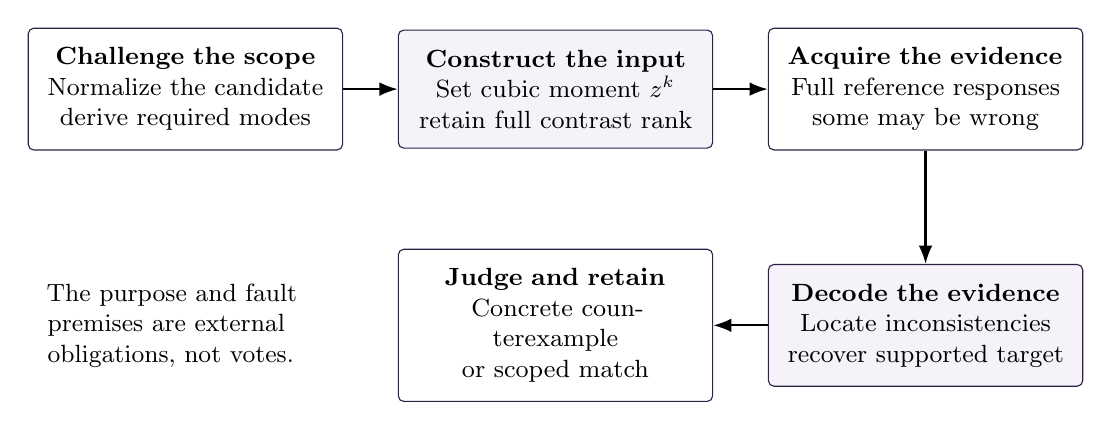
\begin{tikzpicture}[>=Latex,font=\small,box/.style={draw=ink,rounded corners=2pt,align=center,inner sep=7pt,text width=3.5cm,minimum height=1.5cm}]
\node[box] (a) at (0,0) {\textbf{Challenge the scope}\\Normalize the candidate\\derive required modes};
\node[box,fill=wash] (b) at (4.7,0) {\textbf{Construct the input}\\Set cubic moment $z^k$\\retain full contrast rank};
\node[box] (c) at (9.4,0) {\textbf{Acquire the evidence}\\Full reference responses\\some may be wrong};
\node[box,fill=wash] (d) at (9.4,-3.0) {\textbf{Decode the evidence}\\Locate inconsistencies\\recover supported target};
\node[box] (e) at (4.7,-3.0) {\textbf{Judge and retain}\\Concrete counterexample\\or scoped match};
\draw[->,thick] (a)--(b);\draw[->,thick] (b)--(c);\draw[->,thick] (c)--(d);\draw[->,thick] (d)--(e);
\node[align=left,text width=3.5cm] at (0,-3.0) {The purpose and fault\\premises are external\\obligations, not votes.};
\end{tikzpicture}
\caption{The implemented constructive loop. The candidate does not supply its own expected outputs. An audit can request a supported scope extension, but it cannot authorize the necessary experiments or prove its own failure assumptions.}\label{fig:loop}
\end{figure}

\subsection{Preserve the original balanced probes}
Let $V\in\R^{n\times r}$ be a zero-mean full-rank frame whose column cubes sum to zero. Walsh contrast columns provide such a frame at power-of-two $n$; the columns $e_j-e_n$ work at other sizes. The $j$th inherited probe places $V$ in channel block $j$ and zeros elsewhere. Its cubic invariant is zero, and left normalization returns $B_{0,j}$ directly.

Thus the old $k$ probes are systematic coefficient observations of $\Theta_0,\ldots,\Theta_{k-1}$. This paper uses the \emph{actual three inputs and expected outputs} retained from the preceding companion. Their arrays are compared exactly, not merely described as similar. The new moment-shaped inputs are appended to that evidence.

\section{The minimum self-correcting audit}
\label{sec:minimum}
Choose distinct positive rational nodes $z_1,\ldots,z_{q-k}$. The normalized observation matrix is
\begin{equation}
 G=\begin{bmatrix}
 e_0^\top\\ \vdots\\e_{k-1}^\top\\
 v(z_1)^\top\\ \vdots\\v(z_{q-k})^\top
 \end{bmatrix},\qquad
 v(z)=(1,z,z^2,\ldots,z^{K-1})^\top.
 \label{eq:code}
\end{equation}
Each column of a coefficient packet is a scalar channel through this same code. A whole corrupted reference response can alter all packet coordinates simultaneously; no independence across those coordinates is assumed.

\begin{lemma}[Inherited coefficient observations remain full spark]\label{lem:spark}
Every $K$ rows of $G$ are linearly independent when $q\ge K$.
\end{lemma}
\begin{proof}
Take $s$ selected systematic rows and $K-s$ selected positive-node rows. A coefficient vector in their null space defines a polynomial with at most $K-s$ nonzero monomials, because the systematic rows force $s$ coefficients to zero. It also has $K-s$ distinct positive roots. A nonzero real polynomial with $h$ nonzero monomials has at most $h-1$ distinct positive roots: divide by its lowest monomial and apply Rolle's theorem inductively to its derivative. The polynomial must therefore be zero. This proves the claimed rank.
\end{proof}

\begin{theorem}[Minimum fixed-probe correction frontier]\label{thm:main}
For Equation~\eqref{eq:family}, $n\ge4$, $m=k(n-1)$, arbitrary coefficient matrices, and full-output exact reference calls, the minimum number of \emph{fixed} probes needed to identify every target despite at most $t$ arbitrary record corruptions is
\begin{equation}
 \boxed{\quad q^*=k(L+1)+2t=K+2t.\quad}\label{eq:threshold}
\end{equation}
The moment-shaped construction with $k$ inherited balanced probes attains the bound. If those $k$ records remain applicable, exactly $kL+2t$ further calls suffice. These are class-wide, public-audit guarantees, not single-candidate probabilistic detection bounds.
\end{theorem}
\begin{proof}
For necessity, fix any admissible input $X$. With $C=PX$, its response is linear in the unknown coefficients through
\begin{equation}
 [C\ s(C)C\ \cdots\ s(C)^LC].
\end{equation}
This matrix has rank at most $n-1=r$. There are $(L+1)m=rK$ unknown scalar coefficients per output column. If $q<K+2t$, retain at most $q-2t<K$ records; their stacked coefficient equations have rank below $rK$. A nonzero coefficient difference annihilates those records and affects at most the other $2t$. These are genuinely different program maps: Equation~\eqref{eq:poly} supplies identifying inputs for the entire coefficient family. The two-target ambiguity in Theorem~\ref{thm:distance} rules out unique correction. If $q<2t$, the same argument uses an empty retained set.

For sufficiency, Lemma~\ref{lem:spark} says that deleting any $2t$ of the $K+2t$ constructed records leaves full coefficient rank. Therefore two distinct maps disagree on at least $2t+1$ records. Theorem~\ref{thm:distance} supplies unique recovery. Interpolation and full-record residual checking, described below, realize it. Inheriting the $k$ original systematic records leaves $q^*-k=kL+2t$ new queries.
\end{proof}

The additional $2t$ is the familiar error-correction cost. Reed--Solomon codes, coded computing, and resilient estimation already establish the importance of algebraic redundancy \citep{reed,lcc,fawzi}. The specific contribution here is the nonlinear input construction, its compatibility with the predecessor's real probes, and the resulting scope-sensitive audit. The lower bound concerns predetermined probes and a fully arbitrary target in this family. We do not extend it without proof to every adaptive querying strategy, smaller target class, known coefficient specification, or restricted error distribution.

\subsection{Known erasures and unknown corruptions are different resources}
If at most $s$ additional record positions are erased and known to be unusable, the same construction needs $K+2t+s$ positions to tolerate both kinds of failure. Deleting the erasures leaves enough distance to correct the unknown corruptions. A disputed result that has already been reliably identified as unusable can be treated as an erasure; guessing which result is wrong cannot claim that saving. The companion implements complete records and bounded unknown corruptions; an asynchronous erasure-handling service is not implemented.

\subsection{A complete audit is not necessarily the cheapest decision}
An engineer with a trusted complete coefficient table can compare the candidate directly. A single candidate fixed before a fresh random probe can often be rejected without acquiring a deterministic class-wide public audit. Conversely, a public rank-deficient probe set permits an adaptive generator to select an invisible error after seeing its fixtures. The manuscript compares these different obligations rather than prohibiting stronger information or cheaper guarantees to make its own construction look favorable.

\section{Recover the target, then judge the candidate}
\label{sec:decoder}
The runtime first validates the supplied program language and constructs the audit degree and record count. It then recomputes the input frames, normalizes the received outputs, checks the required deletion ranks, and performs error correction. The candidate being judged is not used to decide which reference coefficient vector is true.

A complete but simple decoder enumerates $K$-record subsets, interpolates their coefficient packets, and retains a candidate only if it disagrees with at most $t$ full raw responses. Under the distance condition, at most one such coefficient tuple exists. This method is exponential in the parameters, but transparent for the small checked reference cases.

For the principal $t=1$ study, the implementation uses a standard syndrome locator. It constructs a parity-check matrix $H$ with $HG=0$. A nonzero syndrome component must be proportional to the column of $H$ corresponding to the bad record. Distance at least three ensures that these column directions identify the record uniquely. The runtime then interpolates from unflagged records and verifies the candidate against \emph{every original full output}, including components discarded by row normalization. A corrupt output lying entirely outside the modeled output subspace must not disappear when coordinates are compressed.

\begin{algorithm}[htbp]\small
\caption{Out-Reflect: construct, recover, challenge, and retain}\label{alg:main}
\begin{algorithmic}[1]
\Require Purpose; justified target family; normalized candidate; fault-containment premise; retained reference records
\State Derive the required polynomial scope; do not trust a declared ``linear'' label
\State Construct moment-shaped probes and their deletion-rank obligation
\State Identify which old records retain valid target semantics
\If{the required new reference work is not funded or authorized}
  \State Return a specific evidence obligation; do not report approval
\EndIf
\State Acquire the missing full reference outputs through the actual supported interface
\State Check the declared record or source-group fault model against the design
\State Decode a supported target; otherwise return inconsistency, not a chosen culprit
\State Verify all original record residuals and retain the inconsistent positions
\State Compare the normalized candidate with the recovered target
\State Emit a concrete separating input or a match under the declared premises
\State Archive the scope, reference identity, records, corrections, costs, and invalidation conditions
\end{algorithmic}
\end{algorithm}

The emitted artifact has no operating authority. It binds a reference identity but cannot authenticate that identity's real-world truth. Its reader recomputes the design and decoded target rather than trusting a stored success label. Changing the fault unit from ``reference record'' to ``provider'' is refused; the stronger source-failure claim requires a different audit calculation.

\subsection{When no supported explanation fits}
An inconsistent transcript does not identify which premise failed. Possibilities include too many corrupt records, the wrong target bound, an unrecorded input change, implementation error, or a genuinely changing reference. The system returns \path{INCONSISTENT_WITH_DECLARED_PREMISES}; it does not repair the situation by widening the accepted error budget after observing the answer it prefers.

Conversely, a unique supported fit does not prove those premises. More than $t$ corrupted records can move the transcript within distance $t$ of the wrong map. The explicit beyond-budget experiment below retains exactly that failure.

\section{Executed evidence: an evaluator that survives one wrong reference}
\label{sec:results}
All principal computations use exact rational arithmetic, public or synthetic nonpersonal inputs, and local Python functions. No model provider, remote service, physical apparatus, wallet, or customer is involved. The oracle and candidate implementations use different arithmetic organizations: the reference mixes raw channels and then subtracts means; the candidate centers first and uses a polynomial coefficient evaluation. They share authorship and task premises, not independent institutional validation.

\subsection{The inherited program and the new experiment}
The baseline uses the actual $21\times21$ rational calibration matrix from the preceding artifact. The nonlinear candidate adds $s(C)C$. Its original three inputs and outputs are loaded from the prior package and match the first three new-design records exactly. The new constructor does not receive the calibration matrix as an input; it emits probes from the language bound and dimensions. The published fixture makes the complete coefficients available to readers for reproduction.

The eight-record design contains three old balanced inputs and five coded inputs with nodes $1,2,3,4,5$. It admits degree $L=1$, giving $K=6$ coefficient packets and 882 scalar coefficients. One record contains all 168 output values; eight records therefore contain 1,344 scalar entries before structural dependencies. Describing the result as eight scalar measurements would be false.

The fifth record, at node 2 in the zero-based stored sequence's position 4, is replaced by the nonlinear impostor's entire response. The decoder receives no fault-location hint. It locates position 4 and recovers $(B_*,0)$ exactly. The proposed bad candidate then receives a separating-input record rather than a confidence score.

\subsection{Fault positions, mutations, and fresh reuse}
The driver repeats recovery at every one of the eight record positions under four fault forms: a single entry, a final-row entry, a dense arbitrary perturbation, and a zero-mean perturbation. All 32 cases recover the exact target and locate the altered record. These are artificial fault injections, not empirical frequencies of natural failures.

The signed elementary mutation study covers two coefficient matrices, twenty-one input channels, twenty-one output channels, and both signs: 1,764 errors. All 882 higher-mode signed errors are invisible to the three old probes; every tested error is visible to the completed design. This finite coverage is supporting evidence. The stronger correction guarantee comes from the proved deletion-rank condition, not from treating elementary mutations as a population of all possible faults.

A freshly loaded audit artifact reconstructs its target from the retained received records, including the poisoned one. The resulting implementation agrees with the separate raw-input reference on 64 fresh rational matrices. The fresh task inputs are generated after the construction is fixed in the driver; this is a software confirmation check, not an externally administered or blinded scientific study.

\begin{table}[htbp]\centering\small
\caption{Completed revised-study evidence. A passing software count does not establish a real reference's truth or an error probability.}\label{tab:results}
\begin{tabularx}{\linewidth}{@{}YrY@{}}\toprule
Study & Count & Meaning\\\midrule
Full-response corruption cases & 32 & All eight positions, four injected forms; exact recovery\\
Signed coefficient mutations & 1,764 & 882 nonlinear errors invisible to the inherited fixtures\\
Constructed parameter cases & 54 & Row count, block count, degree, and fault budget varied\\
Independent subset-rank checks & 510 & Every required interpolation subset checked in that grid\\
Independent scalar decoding cases & 80 & Exhaustive interpolation and direct consensus reference\\
Fresh portable input comparisons & 64 & Recovered target agrees with separate raw computation\\
Revised unit-test methods & 52 & Construction, recovery, refusal, lineage, and integrity\\
Predecessor unit-test methods rerun & 52 & Earlier construction preserved; not counted as new experiments\\\bottomrule
\end{tabularx}
\end{table}

\subsection{Strong conventional controls}
A separate scalar-packet reference enumerates all interpolation subsets and directly counts mismatching observations. Across eighty generated domains, including budgets of zero, one, and two corruptions, it finds the same unique target. These tests exercise the coding problem without using the syndrome implementation. They do not compare a rival agent or product, and the scalar reference is not a second independently implemented full numerical runtime.

A conventional specialist given the same nonlinear semantics can construct the same audit and match its minimum. Repeating each of six independent clean-design probes three times would use eighteen records to tolerate one arbitrary global record corruption, versus eight for the constructed code, but that repetition scheme is a diagnostic comparison, not the best specialist alternative. We claim no runtime or scientific superiority over standard coded-computing methods.

The revised method adds an explicit realizable nonlinear probe construction and inheritance mechanism. A generic instruction to use redundancy would not itself supply either. Conversely, naming those constructions ``reflection'' does not make error-correcting codes new.

\section{A successor should extend evidence, not reset its history}
\label{sec:successor}
The probe sequence is independent of the degree it eventually supports. Its first $k$ inputs reveal the base-mode blocks; later inputs use the positive nodes in order. Enlarging $L$ adds coefficients to the polynomial interpretation, not different physical meanings to the already recorded inputs.

\begin{corollary}[Nested scope expansion]\label{cor:inherit}
For an unchanged target and reference semantics, the canonical designs for degrees $L$ and $L+1$ with the same fault budget are nested. Increasing the supported degree by one requires exactly $k$ additional records in this minimum-length construction. Increasing the corruption budget from $t$ to $t+1$ at fixed degree requires two more records. The active fault budget applies to the entire retained transcript, not separately to each generation.
\end{corollary}
\begin{proof}
The total length is $k(L+1)+2t$, the initial systematic rows are unchanged, and new coded nodes append to the same positive-node sequence. Every old input has the same invariant and channel mixture. Its response is therefore unchanged when the target itself is unchanged. The stated length differences follow, and Lemma~\ref{lem:spark} applies to each enlarged interpretation.
\end{proof}

\begin{table}[htbp]\centering\small
\caption{Executed three-generation sequence for one unchanged linear target, with a one-record fault budget maintained throughout. Expanding the candidate class is not changing the target.}\label{tab:lineage}
\begin{tabular}{@{}rrrrr@{}}\toprule
Invariant degree $L$ & Raw degree allowed & Coefficients & New calls & Cumulative calls\\\midrule
0 & 1 & 441 & 5 & 5\\
1 & 4 & 882 & 3 & 8\\
2 & 7 & 1,323 & 3 & 11\\\bottomrule
\end{tabular}
\end{table}

In every generation a corrupted inherited systematic record remains part of the received evidence. Recovery still returns the correct target in the enlarged class. The repeated corruption is the same one bad historical position, not three uncounted fresh errors. Earlier construction costs remain in the cumulative total.

\subsection{A genuinely changed target requires different accounting}
Now authorize a new response $F_{\rm next}(X)=PXB_*+(2/7)s(PX)PX$. Its base-mode calibration is unchanged, so the three balanced records remain valid. The two nonzero-moment records in the five-call linear audit do \emph{not}. Their old expected outputs must be retired.

The new eight-record nonlinear audit consequently reuses three records and obtains five fresh ones. Lifetime reference acquisition is $5+5=10$ calls, not eight. The study checks the valid overlap exactly, rejects the assumption that all prior expected outputs transfer, and recovers the changed target with a bad inherited record still present. Reference identities must change with the intended semantics; array identity alone does not authorize that reassignment.

\insight{\textbf{Reuse the question when it is still useful. Reuse its answer only when its meaning is still valid.}}

\begin{figure}[htbp]\centering
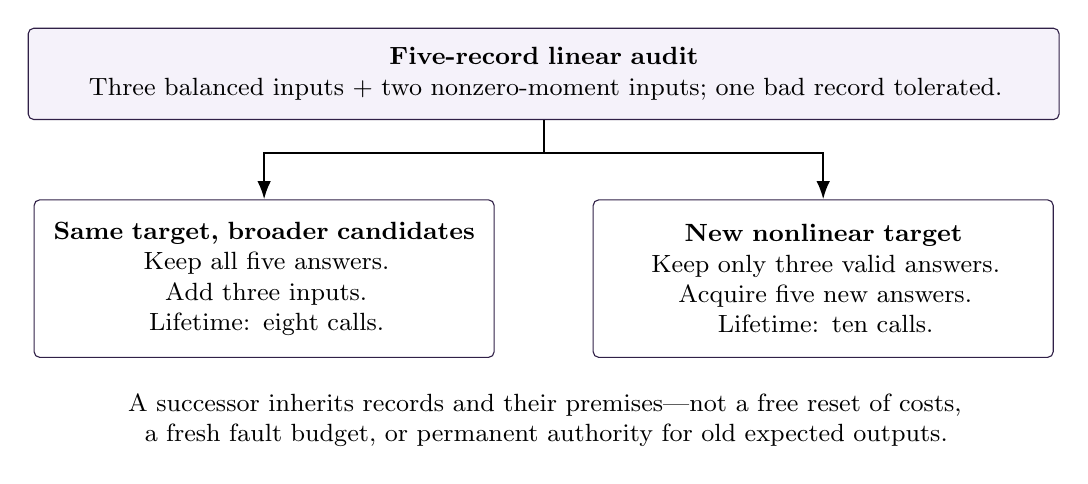
\begin{tikzpicture}[>=Latex,font=\small,box/.style={draw=ink,rounded corners=2pt,align=center,inner sep=7pt}]
\node[box,fill=wash,text width=12.6cm] (a) at (0,0) {\textbf{Five-record linear audit}\\Three balanced inputs + two nonzero-moment inputs; one bad record tolerated.};
\node[box,text width=5.35cm,minimum height=2cm] (b) at (-3.55,-2.6) {\textbf{Same target, broader candidates}\\Keep all five answers.\\Add three inputs.\\Lifetime: eight calls.};
\node[box,text width=5.35cm,minimum height=2cm] (c) at (3.55,-2.6) {\textbf{New nonlinear target}\\Keep only three valid answers.\\Acquire five new answers.\\Lifetime: ten calls.};
\draw[->,thick] (a.south)--(0,-1)-|(b.north);\draw[->,thick] (a.south)--(0,-1)-|(c.north);
\node[align=center,text width=12.8cm] at (0,-4.4) {A successor inherits records and their premises---not a free reset of costs,\\a fresh fault budget, or permanent authority for old expected outputs.};
\end{tikzpicture}
\caption{Two distinct kinds of continuation. Both current nonlinear audits have eight active records. Their historical work and evidence-transfer obligations differ.}\label{fig:inherit}
\end{figure}

\section{The certificate must expose its own failure conditions}
\label{sec:limits}
\subsection{One fewer record permits two incompatible explanations}
With $q=K+2t-1$, a full-spark design has two targets differing in only $2t$ records. A transcript can then be within $t$ corruptions of both. The companion constructs an exact small example with two targets and one corrupted record under either explanation. No vote, additional reflection over the same transcript, or tie-breaking convention can make a universal verdict valid.

The loader refuses insufficient redundancy even when all currently supplied values happen to fit one target. Existence of a clean-looking fit is not the distance guarantee required for future arbitrary errors.

\subsection{Too many errors can manufacture a uniquely wrong answer}
At the sufficient length for $t=1$, the code has minimum distance three. The study constructs two targets whose clean transcripts differ in three positions. A received transcript is one error away from target A and two errors away from target B. Under the asserted one-error model, the correct mathematical decoder chooses A. If B was the real target and two records were corrupted, the conclusion is wrong.

The reference does not detect every violation of its own budget. This counterexample is retained explicitly. A proof conditional on one corruption cannot be promoted into an observed guarantee that at most one corruption occurred.

\subsection{A coherent wrong reference is not corrected by agreement}
If all reference outputs are generated by the same wrong transformation, they form a clean codeword. The decoder recovers that transformation with no inconsistent records. This is reproduced with the nonlinear impostor as the shared reference. The source-group audit correctly rejects a one-source-failure guarantee for that arrangement, but no algebraic check authenticates which transformation the user truly intended.

The revised contribution is \emph{bounded corruption correction}, not truth without an anchor. A lawful specification, measured calibration, or independently justified reference process still determines the target. Error-correcting experimental design can reduce dependence on each individual result; it cannot eliminate every trusted premise.

\subsection{A larger language can hide a new error again}
The current public probe set has finitely many cubic-invariant values $a_1,\ldots,a_h$. Define
\begin{equation}
 \widetilde F(X)=F_*(X)+\left[\prod_{j=1}^{h}\bigl(s(PX)-a_j\bigr)\right]PX.
\end{equation}
It agrees with every retained probe and differs elsewhere. In the eight-record anchor there are six distinct invariant values, including zero. This term has invariant degree six and lies outside the degree-one audit. The companion executes the agreement and a fresh counterexample; the program normalizer would request a scope extension rather than reuse the old certificate.

The example makes open-ended self-certification impossible from a fixed finite transcript without additional restrictions. The constructive result is not that no future blind spot exists. It is that a supported class enlargement has an explicit cost and a generated experiment, instead of an unexamined confidence label.

\subsection{Exact correction does not make finite precision free}
Let $G$ be the normalized audit matrix and, at the minimum record count, define
\begin{equation}
 \beta_t=\max_{|S|=q-2t}\|G_S^{-1}\|_\infty,\qquad
 \lambda=\max_i\|\Lambda_i\|_\infty.
\end{equation}
Suppose two coefficient fits each disagree arbitrarily with at most $t$ records and fit every entry of all remaining raw responses within $\eta$. Their good-record sets overlap on at least $K$ positions. Normalization changes entry errors by at most $\lambda$, so on such a subset,
\begin{equation}
 \|\widehat\Theta-\Theta\|_{\max}\le2\beta_t\lambda\eta.\label{eq:noise}
\end{equation}
Here $\|\cdot\|_{\max}$ is the largest absolute scalar coefficient. This is a conditional stability consequence, not a noise distribution or a numerical implementation certificate.

For the exact anchor, all twenty-eight six-record inverse norms are computed. The worst is $\beta_1=80/3$. The largest normalizer norm is $189012/63379$, giving a coefficient-entry difference bound of $(10080640/63379)\eta$, approximately $159.05\eta$. The input-to-feature construction can therefore be much more delicate than its small probe count suggests. The executable decoder uses exact rational arithmetic; a robust noisy decoder and physical error calibration remain unimplemented.

\section{Relationship to prior art: the advantage must survive an honest comparison}
\label{sec:prior}
Error-correcting codes deliberately add algebraic redundancy so that wrong symbols can be detected or corrected \citep{reed}. Lagrange Coded Computing extends polynomial evaluation to tolerate stragglers and Byzantine workers \citep{lcc}. Secure estimation characterizes recovery under sparse malicious measurements \citep{fawzi}. These precedents already establish that multiple faulty results need not make every computation impossible. This paper does not claim to originate that principle or the $2t$ term.

The specific scientific problem differs from ordinary delivery of encoded data. Our target coefficients are unknown, a reference accepts input matrices rather than arbitrary desired code symbols, and its response includes a nonlinear global cubic invariant. The moment-shaped frame constructs inputs realizing a univariate packet polynomial while leaving inherited balanced observations usable. Its proof, minimum fixed-probe count, and exact lineage are the technical center of this revision. Equivalent specializations may exist elsewhere; the targeted review does not establish universal priority.

The oracle problem in software testing is also longstanding \citep{oracle}. Metamorphic properties can be necessary without identifying the intended output. The first edition's mean--contrast structure is an application of established permutation-equivariant linear algebra \citep{deepsets,reflect1}. Here those previous guarantees are retained for their class, not retroactively called false. The change is to support a richer class and a weaker per-record trust requirement.

\begin{table}[htbp]\centering\small
\caption{What is inherited, what is constructed, and what remains outside the claim. No named external system is benchmarked here.}\label{tab:prior}
\begin{tabularx}{\linewidth}{@{}P{.23\linewidth}YY@{}}\toprule
Foundation & Established capability & This revision's specific role\\\midrule
Error-correcting codes & Recover data under bounded symbol corruption & Make actual nonlinear reference experiments produce a decodable packet code\\
Coded computing & Encode computation to tolerate faulty workers & Unknown coefficient identification with reusable predecessor probes\\
Secure estimation & Identify states despite corrupted measurements & Purpose-relative and source-group audit conditions\\
Metamorphic testing & Check relationships among executions & Expose a nonlinear term invisible on the old symmetric fixtures\\
Agent reflection & Use feedback to revise behavior, prompts, or answers & A deterministic evidence constructor, not a learned reflective policy\\\bottomrule
\end{tabularx}
\end{table}

Reflexion uses verbal feedback and retained experience; Self-Refine iterates generation and critique; CRITIC introduces tool-interactive checking \citep{reflexion,selfrefine,critic}. SCoRe learns multi-turn correction behavior, while GEPA uses reflection to evolve prompts \citep{score,gepa}. These are relevant proposal mechanisms, not competitors defeated by a small exact algebraic experiment. Our system neither measures their performance nor establishes that contemporary models cannot self-correct.

AlphaEvolve's generated programs and automated evaluators could propose a better moment frame, a stronger supported language, or a more efficient decoder \citep{alphaevolve}. The research opportunity is complementary: make an evaluator's actual information and trust assumptions editable and checkable, rather than infer them from the persuasive quality of an improvement narrative.

\section{A reflective capability for SUCCESSOR \texorpdfstring{$\Omega$}{Omega}}
\label{sec:successor_system}
The implementation target remains \href{https://github.com/MontrealAI/AGI-Alpha-Agent-v0}{AGI Alpha Agent / SUCCESSOR $\Omega$}. The current deliverable is a local research adapter; no repository integration or release is claimed.

The proposed project record separates the intended result, candidate program class, reference semantics, actual input--output records, fault-containment model, decoding evidence, and authorization. That separation makes the following product states meaningful: \emph{unsupported candidate scope}; \emph{missing reference work}; \emph{inconsistent premises}; \emph{recovered under stated fault assumptions}; \emph{candidate contradicted}; and \emph{candidate matches within scope}. None is a universal success badge.

The original thought experiment about a second model finding a missing chapter remains useful. Its lesson is not simply that two models are better than one. The second process helps when it introduces a distinction the first process failed to examine. In the present construction, that distinction is engineered through probes and a code. For an actual book, factual coverage, importance, source access, and reader purpose would need a different evidence model; the polynomial theorem does not transfer by metaphor.

\subsection{A new kind of inherited asset}
The enduring artifact is not the critic's explanation. It is a tested method for producing and interpreting evidence, together with a record of what could still make that interpretation wrong. Out-Think can carry a supported representation; Out-Strategise can select what to investigate; Out-Execute can preserve evidence through interruption; Out-Reflect can expose and repair a supported weakness in that evidence. Their titles do not establish a completed end-to-end integration.

A system that later proposes a better audit should compare complete campaigns with matched initial records, model access, tool permissions, human intervention, and reference budgets. A larger archive is an asset, not proof of improved discovery. Discovering the correct nonlinear class or a trustworthy failure model from an unfamiliar task remains substantially harder than solving the supplied one.

\subsection{The next natural experiment}
An appropriate pilot would use an independently chosen benign scientific-software workflow with a real family of numerical transformations, costly reference evaluations, and a documented failure-containment model. Competing specialists and agents should be allowed to inspect specifications, change probe designs, use established coding tools, and decline unsupported assurances. The winning frame must not be handed to only one arm.

Measure whether the proposed reflection finds a consequential evaluator limitation, constructs feasible evidence, locates injected faults selected outside the method, and preserves correct conclusions after a genuinely different task or implementation. Count formalization, failed search, precision, engineering, source diversification, decoding, and review. Report numerical reliability, semantic correctness, adoption, and commercial acceptance separately. That study has not been performed here.

\section{Invent the economy around evidence worth using}
\label{sec:economy}
The commercial object is a \emph{qualified evidence-construction capability}, not more favorable verdicts. A sponsor might fund a bounded investigation of an expensive scientific or software evaluator, followed by separately accepted deployment if a supported audit can be built. An honest negative result can complete the research phase without being sold as a working assurance product.

\emph{Invent the Economy} makes the capability and the arrangement jointly editable \citep{economy}. Here the connection is operational. A buyer requiring one specified answer may need a three-record purpose-only check. A buyer requiring repeated public qualification of arbitrary supported candidates needs the larger class-wide audit. A buyer requiring tolerance of one \emph{provider} failure needs enough source-separated evidence; eight records from a shared fragile service do not meet that promise. Accepted assurance scope changes which construction must be financed.

The elementary call-count advantage over repeated individual probes is real within its stated comparison. For $K$ independent coefficient packets and $t$ arbitrary global bad records, protecting every separate packet by $2t+1$ repetitions uses $K(2t+1)$ calls. The constructed code uses $K+2t$, a difference of $2t(K-1)$. But constructing difficult inputs, higher precision, source access, and decoding may cost more than those saved calls. An unrestricted coding specialist can match the latter count.

Let $F$ include discovery, model justification, failed attempts, source qualification, and implementation. Let $c_i$ be the actual acquisition cost of each accepted reference record, and $D_j$ the complete subsequent audit, integration, storage, and maintenance burden. A same-quality offer is economical only if
\begin{equation}
 F+\sum_i c_i+\sum_j D_j<C_{\rm best\ supported\ alternative}.
\end{equation}
There are no invented prices or revenues in this paper. Distinct nonlinear modes are not automatically distinct businesses. Actual beneficiaries must accept actual outputs and terms. Future payments do not finance earlier work unless funds are genuinely available under their obligations.

MONTREAL.AI retains parent ownership as a design constraint. Public mathematics and open code do not become exclusive property by being entered into a registry. A commercial advantage would need qualified execution, useful adapters, lawful reuse rights, reliable delivery, and continuing effective discovery. Copying and stronger conventional tools can reduce that advantage.

The inherited USDC and \$AGIALPHA routes remain separate. This manuscript changes no token-holder right, contract, fee, wallet, or deployment permission, and derives no token valuation. A useful audit may eliminate unnecessary model calls and should be permitted to do so. Creating artificial review activity to sustain fees would oppose the capability's purpose.

The larger productive pathway is conditional but concrete: better evidence supports a genuinely useful capability; accepted applications earn resources after obligations; those resources fund another capability or productive asset. Reflection contributes by making unreliable premises visible and, in supported cases, correctable. It does not turn an algebraic result into industrial capacity by declaration.

\section{Conclusion: construct a mirror that can survive a crack}
The first edition asked what a judge could not see. This revision asks what must be constructed when the answer lies outside its old class and one of the answers used to judge it may be wrong.

The response is executable. A normalized program determines a bounded nonlinear scope. Moment-shaped inputs transform that scope into a polynomial observation code. An exact distance condition supplies the minimum fixed audit length. A decoder recovers the target, localizes inconsistent records, and produces a concrete candidate counterexample. A successor retains valid evidence, expands supported scope, and preserves the difference between a broader candidate language and a changed target.

The anchor is not a universal reflective intelligence. It is a precise advance beyond the predecessor's positive guarantee: a previously excluded nonlinear failure is supported, a bounded corrupt reference is corrected, and the costs and limits of subsequent evidence inheritance are explicit. The construction preserves rather than weakens the purpose.

\insight{\textbf{The strongest reflection does not merely explain why a result should be trusted. It constructs evidence that can expose---and within its scope correct---the errors on which that trust depends.}}

\Needspace{10\baselineskip}
\section*{Research status}
This AI-assisted research manuscript reports written mathematical proofs, an exact local computational construction, and synthetic fault and scope-change experiments. The separate implementations share authorship; there is no external peer review or proof-assistant formalization. No live language-model discovery campaign, physical calibration, remote-provider trial, signed customer, revenue, token-price experiment, or production integration is claimed. The original artifacts remain unchanged. This revision's claims apply to its actual code, results, and stated premises.

\par\bigskip
\appendix
\section{Proof details and complete accounting}
\label{app:proofs}
\subsection{Why the nonlinear coefficient family is identifiable}
A possible concern in the dimension lower bound is whether two different coefficient tuples could describe the same nonlinear program. The constructed inputs resolve this. If the difference map is identically zero, Equation~\eqref{eq:poly} is the zero matrix polynomial for every positive rational $z$. Every coefficient packet is therefore zero. Thus the family has $(L+1)m^2$ independent scalar coefficients as a function class, and a nonzero coefficient null vector in Theorem~\ref{thm:main} genuinely describes a different target.

The dimension bound can be stated without packet notation. One output column has $(L+1)m$ unknown coefficients. Each centered input contributes at most $r=n-1$ independent equations for that column because the repeated scalar-mode blocks all have the same column space as $C$. Fewer than $K$ retained reference inputs cannot identify that column for every target. Deletion of $2t$ positions is necessary for arbitrary $t$-record correction by the two-transcript argument. The constructor attains that obstruction's removal through its particular nonlinear input interface.

\subsection{Why the mixed systematic--evaluation matrix is full spark}
Fix a nonzero polynomial $p(z)$ with $h$ nonzero monomials and divide by its smallest power of $z$. The resulting function has a nonzero constant term. Its derivative has at most $h-1$ nonzero monomials. By induction it has at most $h-2$ distinct positive zeros, so Rolle's theorem allows the original at most $h-1$. The base case is a single nonzero monomial, which has no positive zero. This argument needs no generic-position or probabilistic claim about the chosen nodes.

A selected systematic row forces one monomial coefficient to zero. If $s$ such rows are selected among $K$ observations, the remaining polynomial has at most $K-s$ nonzero terms but would need $K-s$ positive roots from the selected evaluation rows. It is zero. Positivity is substantive: arbitrary signed nodes can create singular generalized evaluation submatrices.

\subsection{A left normalization is not a license to ignore output coordinates}
For a supported clean output, $Y=WZ$ and any left inverse returns $Z$. A corrupted output can have a component outside the column space of $W$. That component may disappear under normalization. The implementation therefore always reconstructs each \emph{entire} raw response from the decoded coefficients and compares it with the received matrix. Correcting the normalized symbols alone would not justify a claim that no original record was inconsistent.

The study includes final-row and nonzero-mean corruptions as well as the centered impostor response. The first two are not the hard headline case, but they ensure that a projection cannot hide a fault from the reported correction record.

\subsection{Error domains and the cost of a new generation}
If the fault model permits any $t$ bad record positions, the same historical position stays one fault when reused. Newly acquiring another response creates another position and can introduce another error; a per-generation budget cannot be combined into a lifetime bound by resetting its name. The lineage experiment explicitly carries one bad inherited record throughout and makes no claim about additional uncounted errors.

For source-group failures, delete the union of every pair of permitted source-failure sets. If an output-relevant coefficient difference survives only on deleted records, two differently corrupted targets can explain the same received evidence. The package returns such a rank deficiency and a coefficient witness. A passing supplied group model still needs evidence that the physical fault domains are correctly described.

\section{Reproduction and actual source custody}
\label{app:repro}
The package uses Python's standard library: rational arithmetic, JSON, hashing, and deterministic combinatorial operations. The recorded runtime uses Python 3.13.5 on Linux. Scripts write only their own research-package inputs and results. They require no network credentials, paid API, GPU, wallet, model service, or external database.

\begin{lstlisting}
python -S code/run_study.py
python -S -m unittest discover -s tests -v
xelatex -no-shell-escape -interaction=nonstopmode \
  -halt-on-error Out_Reflect_Revised.tex
xelatex -no-shell-escape -interaction=nonstopmode \
  -halt-on-error Out_Reflect_Revised.tex
\end{lstlisting}

The query utility reads the retained capsule and a bounded candidate program. Its reference identity must be supplied explicitly. It returns a scoped match, a counterexample, or a request for a broader audit; it does not contact the reference source or authorize an action. The data-only parser is bounded but is not claimed as a complete hostile-input security audit.

\begin{table}[htbp]\centering\small
\caption{Principal revised artifacts. The original paper is preserved separately, not silently overwritten.}\label{tab:files}
\begin{tabularx}{\linewidth}{@{}P{.42\linewidth}Y@{}}\toprule
Artifact & Role\\\midrule
\path{code/construction.py} & Moment-shaped probes, code construction, decoding, source-group audit\\
\path{code/model.py} & Bounded program normalizer and candidate evaluator\\
\path{code/reference.py} & Raw-input reference and separate exhaustive scalar decoder\\
\path{code/query_audit.py} & Data-only candidate inspection against the portable audit\\
\path{inputs/predecessor.json} & Actual original probes, expected outputs, and reference coefficients\\
\path{results/audit_capsule.json} & Portable received transcript, including its corrupted record\\
\path{results/succession.json} & Three-generation costs and changed-target non-reuse\\
\path{results/source_faults.json} & Record versus provider failure-domain counterexamples\\
\path{results/limits.json} & Insufficient distance, excess corruption, common-mode and degree failures\\
\path{tests/test_revision.py} & Fifty-two revised functional and boundary test methods\\\bottomrule
\end{tabularx}
\end{table}

The original LaTeX, contribution note, and skeptical review were read in full. Their checksums and the original ZIP identity are recorded in \path{sources/predecessor_manifest.json}. The earlier test suite was run in a separate extraction and all 52 methods passed. That is a reproduced predecessor check, not an additional 52 new experiments. The new package retains the prior source and real probe records while rebuilding the main argument around a different positive guarantee.

The generated confirmation inputs record seeds, complete cases, and source hashes. They are author-generated software checks, not independent preregistration or evidence about a natural task population. Raw timings exclude mathematics, research, software authoring, review, compilation, and integration. Deterministic semantic outputs are hashed separately from environment and elapsed-time records.

The complete revised driver invokes the separate raw reference routine 143 times, including repeated truth checks, fault controls, fresh-input comparisons, and successor checks. That total is distinct from the eight logical acquisition records in the anchor or the cumulative acquisition totals of 5, 8, and 11 along one lineage. No test-harness work is claimed to disappear. All quantities in the minimum theorem count full reference calls. The scalar output width, coefficient dimension, exact arithmetic cost, conditioning, normalization, and source qualification remain separate. The small runtime does not establish saved human work, reduced model tokens, lower energy consumption, or a commercial margin.

\subsection{Research cutoff and priority boundary}
External primary sources were checked through 21 October 2026. The paper uses the published foundations of coding, coded computing, secure estimation, program testing, and reflective agents. It does not import unverified product rankings from previous drafts. The reference comparison is targeted, not an exhaustive novelty search. In particular, a specialist may identify equivalent moment constructions or experimental-code specializations. The contribution stands on its explicit construction, proofs, and reproducible consequences, not on an unsupported claim of firstness.

The standalone LaTeX embeds all vector figures, tables, and references. It uses locally installed Noto Serif, Noto Sans, and DejaVu Sans Mono. No font files are distributed. The original foundation papers, repository branches, releases, deployments, and financial settings remain unchanged.

\clearpage
\section{Claim--evidence register}
\small
\begin{longtable}{@{}P{.28\linewidth}P{.33\linewidth}P{.32\linewidth}@{}}\toprule
Claim & Evidence & Boundary\\\midrule\endfirsthead
\toprule Claim & Evidence & Boundary\\\midrule\endhead
Bounded wrong records can be corrected & Purpose-relative distance criterion; exact recovery studies & True target and fault-containment premises remain external\\
A nonlinear response can realize the required code & Explicit moment-frame lemma and Equation~\eqref{eq:poly}; exact input checks & Named polynomial family, signed rational inputs, $n\ge4$, $m=k(n-1)$\\
$K+2t$ fixed reference calls are minimum & Rank/deletion lower bound and full-spark construction & Fixed probes, arbitrary coefficient family, vector-valued exact observations\\
Old three probes are actually reused & Exact arrays and expected-output agreement with prior artifact & Only unchanged or explicitly compatible reference semantics\\
Nonlinear impostor and a corrupt reference are handled together & Eight-record anchor, exact 882-coefficient recovery & One bad record, not an arbitrary faulty source\\
Correction works at every tested position & 32 actual artificial record faults & Not a natural error-rate estimate or distributed provider trial\\
The design generalizes across selected parameters & 54 cases; 510 independent rank checks & One authored mathematical family\\
Independent conventional decoder ties & 80 exhaustive scalar-packet cases & Not a head-to-head benchmark against named AI systems\\
Successors add valid scope without rewriting cost & Five/eight/eleven-call lineage and ten-call changed-target case & No learned improvement policy or automatic semantic migration\\
A unique fit establishes reference truth & Explicitly false; common-mode and excess-fault counterexamples & No universal self-authentication\\
A noisy physical audit is implemented & Not claimed; conditional exact sensitivity bound only & Calibration, finite-precision decoder, and deployment remain future work\\
A valuable business is established & Not claimed; mechanism-derived service and cost conditions & No actual buyer, price, receipt, valuation, or operational grant\\\bottomrule
\end{longtable}
\normalsize

\clearpage
\begin{thebibliography}{99}
\footnotesize\raggedright\setlength{\itemsep}{.13em}\setlength{\parsep}{0pt}
\bibitem[Agrawal et~al.(2026)]{gepa}
Lakshya A. Agrawal et~al. \emph{GEPA: Reflective Prompt Evolution Can Outperform Reinforcement Learning}. arXiv:2507.19457v2, 14 February 2026. \url{https://arxiv.org/abs/2507.19457v2}.
\bibitem[Barr et~al.(2015)]{oracle}
Earl T. Barr, Mark Harman, Phil McMinn, Muzammil Shahbaz, and Shin Yoo. The oracle problem in software testing: A survey. \emph{IEEE Transactions on Software Engineering}, 41(5):507--525, 2015. \url{https://doi.org/10.1109/TSE.2014.2372785}. Author repository: \url{https://discovery.ucl.ac.uk/1471263/}.
\bibitem[Boucher(2026a)]{transform}
Vincent Boucher. \emph{Transformational Intelligence: Learning to Change the Game}. MONTREAL.AI research manuscript, October 2026. Retained research foundation. \url{https://github.com/MontrealAI/AGI-Alpha-Agent-v0/blob/main/docs/Transformational_Intelligence.pdf}.
\bibitem[Boucher(2026b)]{economy}
Vincent Boucher. \emph{Invent the Economy: Transformational Intelligence for Creating Viable Markets}. MONTREAL.AI research manuscript, October 2026. Retained foundation; no new commercial evidence inferred. \url{https://github.com/MontrealAI/AGI-Alpha-Agent-v0/blob/main/docs/Invent_the_Economy.pdf}.
\bibitem[Boucher(2026c)]{strategy}
Vincent Boucher. \emph{Out-Strategise: Transformational Intelligence for Constructing the Conditions of Success}. MONTREAL.AI, 20 October 2026. Retained source. \url{https://github.com/MontrealAI/AGI-Alpha-Agent-v0/blob/main/docs/Out_Strategise.pdf}.
\bibitem[Boucher(2026d)]{execute}
Vincent Boucher. \emph{Out-Execute: Transformational Intelligence for Making Progress Survive}. MONTREAL.AI, 21 October 2026. Retained source; no fresh release claim.
\bibitem[Boucher(2026e)]{think}
Vincent Boucher. \emph{Out-Think: Transformational Intelligence for Inventing the Space of Reasoning}. MONTREAL.AI, 21 October 2026. Retained complete source. \url{https://github.com/MontrealAI/AGI-Alpha-Agent-v0/blob/main/docs/Out_Think.pdf}.
\bibitem[Boucher(2026f)]{reflect1}
Vincent Boucher. \emph{Out-Reflect: Transformational Intelligence for Discovering What Its Own Checks Cannot See}. MONTREAL.AI, 21 October 2026, preceding edition. Complete supplied LaTeX, contribution note, review, and executable package; exact identities in the companion. Preserved, not overwritten.
\bibitem[Fawzi et~al.(2014)]{fawzi}
Hamza Fawzi, Paulo Tabuada, and Suhas Diggavi. Secure estimation and control for cyber-physical systems under adversarial attacks. \emph{IEEE Transactions on Automatic Control}, 59(6):1454--1467, 2014. Author preprint: \url{https://arxiv.org/abs/1205.5073}. Inspected record and conditional recovery criterion.
\bibitem[Gou et~al.(2024)]{critic}
Zhibin Gou, Zhihong Shao, Yeyun Gong, Yelong Shen, Yujiu Yang, Nan Duan, and Weizhu Chen. \emph{CRITIC: Large Language Models Can Self-Correct with Tool-Interactive Critiquing}. arXiv:2305.11738v4, revised 21 February 2024. \url{https://arxiv.org/abs/2305.11738v4}.
\bibitem[Kumar et~al.(2024)]{score}
Aviral Kumar et~al. \emph{Training Language Models to Self-Correct via Reinforcement Learning}. arXiv:2409.12917v2, revised 4 October 2024. \url{https://arxiv.org/abs/2409.12917v2}.
\bibitem[Madaan et~al.(2023)]{selfrefine}
Aman Madaan et~al. \emph{Self-Refine: Iterative Refinement with Self-Feedback}. arXiv:2303.17651v2, 25 May 2023. \url{https://arxiv.org/abs/2303.17651v2}.
\bibitem[Novikov et~al.(2025)]{alphaevolve}
Alexander Novikov et~al. \emph{AlphaEvolve: A Coding Agent for Scientific and Algorithmic Discovery}. arXiv:2506.13131, 16 June 2025. \url{https://arxiv.org/abs/2506.13131}.
\bibitem[Reed and Solomon(1960)]{reed}
I. S. Reed and G. Solomon. Polynomial codes over certain finite fields. \emph{Journal of the Society for Industrial and Applied Mathematics}, 8(2):300--304, 1960. \url{https://doi.org/10.1137/0108018}. The present experiments use exact rational arithmetic, not a claim to extend the original finite-field theory.
\bibitem[Shinn et~al.(2023)]{reflexion}
Noah Shinn, Federico Cassano, Edward Berman, Ashwin Gopinath, Karthik Narasimhan, and Shunyu Yao. \emph{Reflexion: Language Agents with Verbal Reinforcement Learning}. NeurIPS 2023; arXiv:2303.11366. \url{https://arxiv.org/abs/2303.11366}.
\bibitem[Yu et~al.(2019)]{lcc}
Qian Yu, Songze Li, Netanel Raviv, Seyed Mohammadreza Mousavi Kalan, Mahdi Soltanolkotabi, and Salman A. Avestimehr. Lagrange coded computing: Optimal design for resiliency, security, and privacy. \emph{Proceedings of Machine Learning Research}, 89:1215--1225, 2019. \url{https://proceedings.mlr.press/v89/yu19b.html}. Open preprint: \url{https://arxiv.org/abs/1806.00939}.
\bibitem[Zaheer et~al.(2017)]{deepsets}
Manzil Zaheer, Satwik Kottur, Siamak Ravanbakhsh, Barnabás Póczos, Ruslan Salakhutdinov, and Alexander Smola. \emph{Deep Sets}. NeurIPS 2017; arXiv:1703.06114. \url{https://arxiv.org/abs/1703.06114}.
\end{thebibliography}
\end{document}
